
\documentclass[12pt,palatino]{bppaper}
\usepackage{blindtext}

%%%%%%%%%%%%%%%%%%%%%%%%%%%%%%%%%%%%%%%%%%

\title{Title of the project}
\author{Author's name 1\\Institution 1 \and Author's name 2\\Institution 2}
\date{\today}
%\abstract{\blindtext}
\jel{jel1, jel2, jel3}
\keywords{keyword1, keyword2, keyword3}
%\thanks{\blindtext}

%%%%%%%%%%%%%%%%%%%%%%%%%%%%%%%%%%%%%%%%%%

\begin{document}
\maketitle

%%%%%%%%%%%%%%%%%%%%%%%%%%%%%%%%%%%%%%%%%%

\section{First section's heading}

\blindtext

\paragraph{Paragraph heading}
\blindtext
$$e^{\pi i} - 1 = 0$$
\blindtext Example of footnote.\footnote{\blindtext}
\begin{equation}
    ax^2 +b x + c = 0 \so \llave{x = \dfrac{-b \pm \sqrt{b^2 - 4ac}}{2a}}{Solution}
\end{equation}

\section{Third section's heading (with table and figure)}

\blindtext

\subsection{Subsection heading, with a table}

\blindtext
\begin{table}[t]
\centering
\caption{Heading of the table, with \texttt{[t]}}
\begin{tabular}{cccc} \toprule
    & Mean & Median & Std Desvi.\\ \midrule
    Variable 1 & $1150$ & 900 & 235 \\ 
    Variable 2 & $430$ & 300 & 57 \\ 
    Variable 3 & $367$ & 210 & 113 \\ \bottomrule
\end{tabular}
\end{table}
\blindtext

\blindtext
\begin{table}[h]
\centering
\caption{Heading of the table, with \texttt{[h]}}
\begin{tabular}{cccc} \toprule
    & Mean & Median & Std Desvi.\\ \midrule
    Variable 1 & $1150$ & 900 & 235 \\ 
    Variable 2 & $430$ & 300 & 57 \\ 
    Variable 3 & $367$ & 210 & 113 \\ \bottomrule
\end{tabular}\par
\end{table}
\cite{lesk:1977}.
\blindtext

\subsection{Subsection heading, with a figure}

\blindtext \cite{knuth:1984}.
\begin{figure}[h!]
\centering
\caption{Heading of the figure, with \texttt{[h]}}
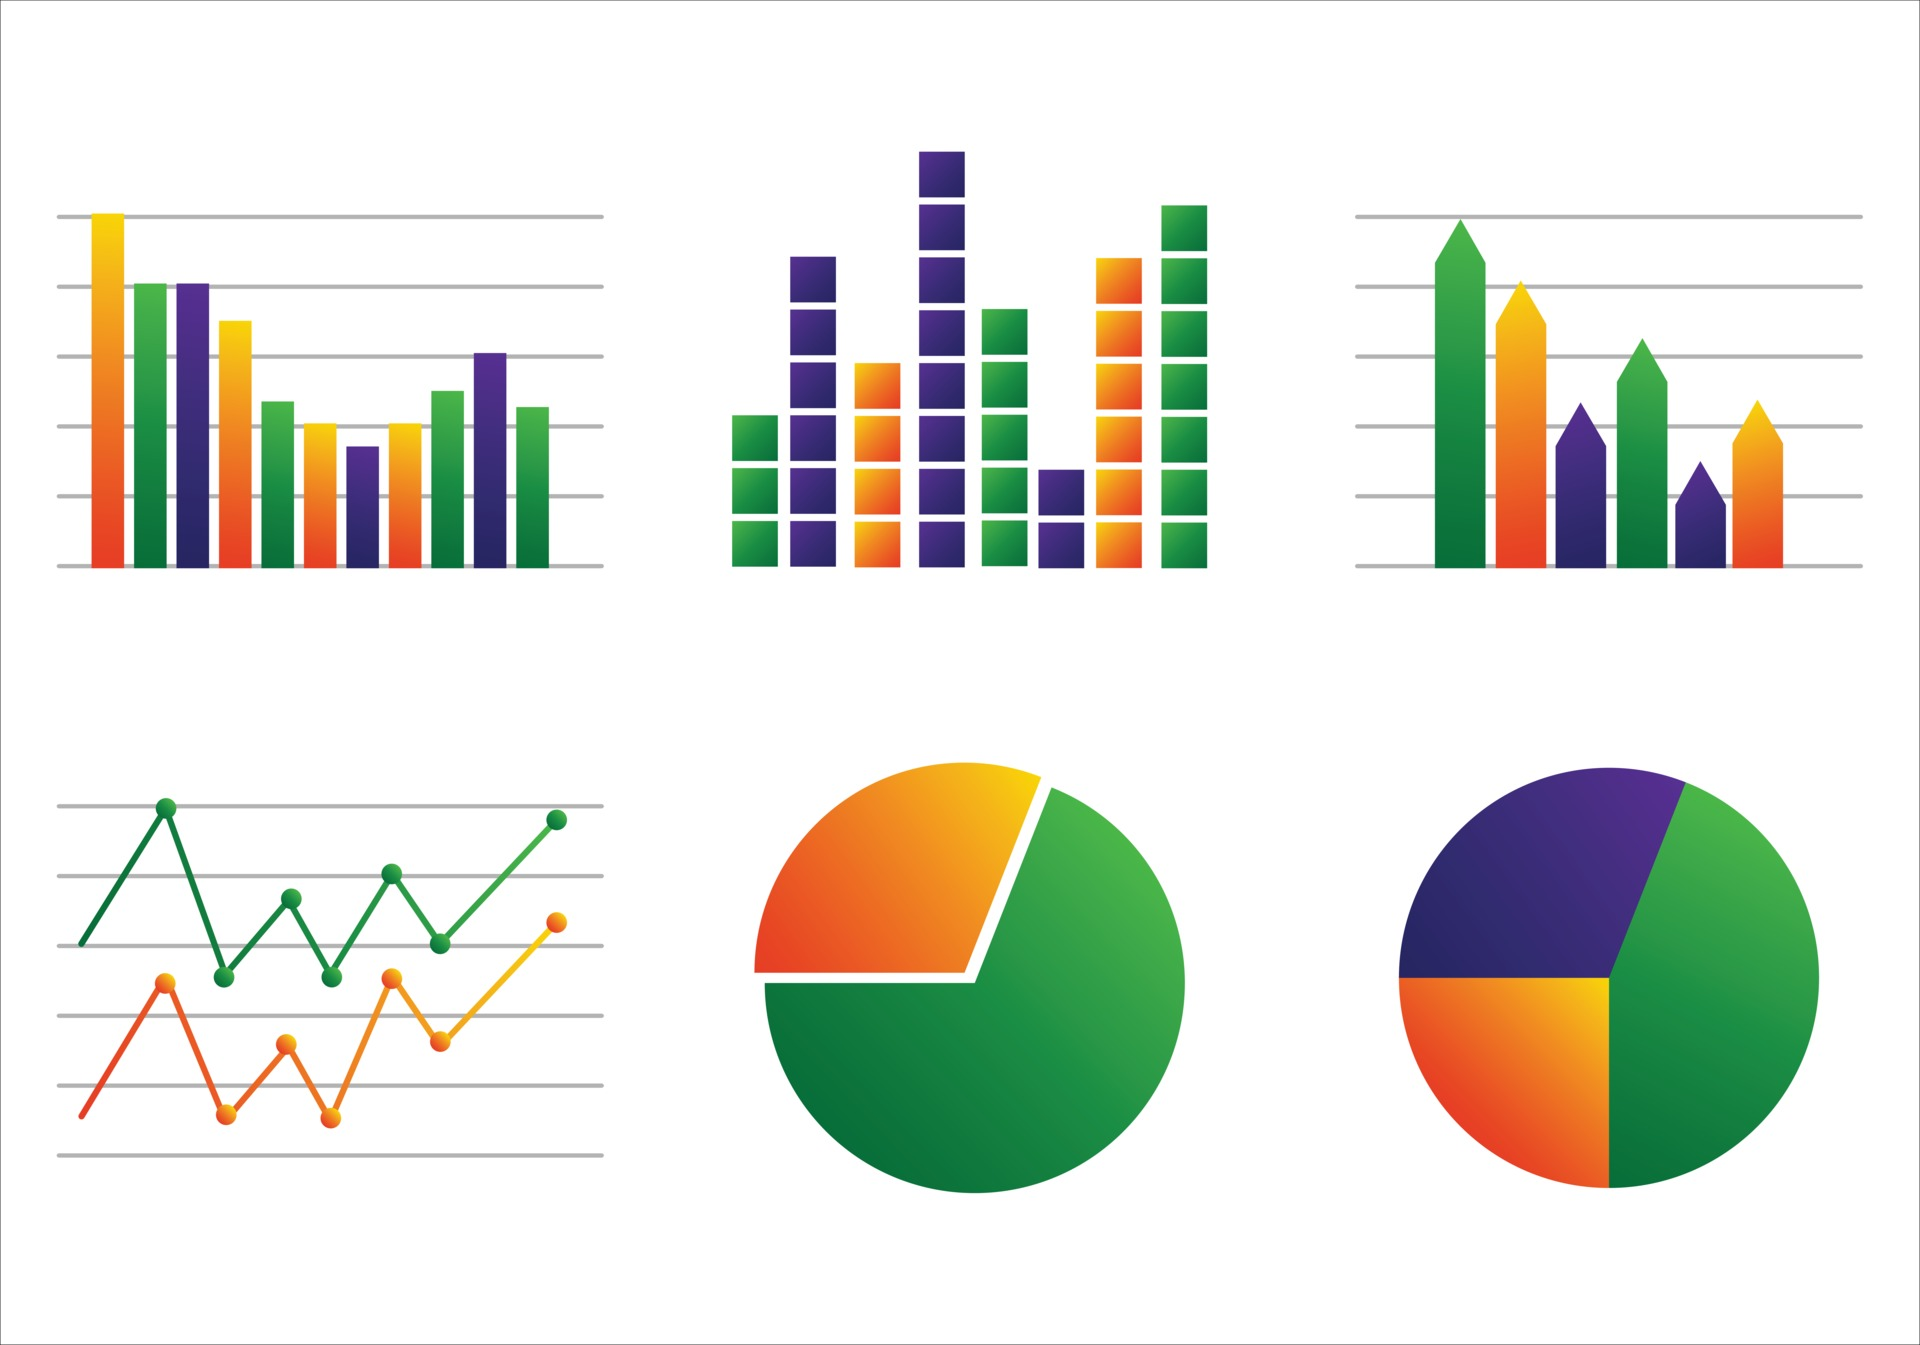
\includegraphics[width=0.8\linewidth]{graph}
\end{figure}
\cite{latex:companion}. \blindtext 

\blindtext
\begin{figure}[t]
\centering
\caption{Heading of the figure, with \texttt{[t]}}
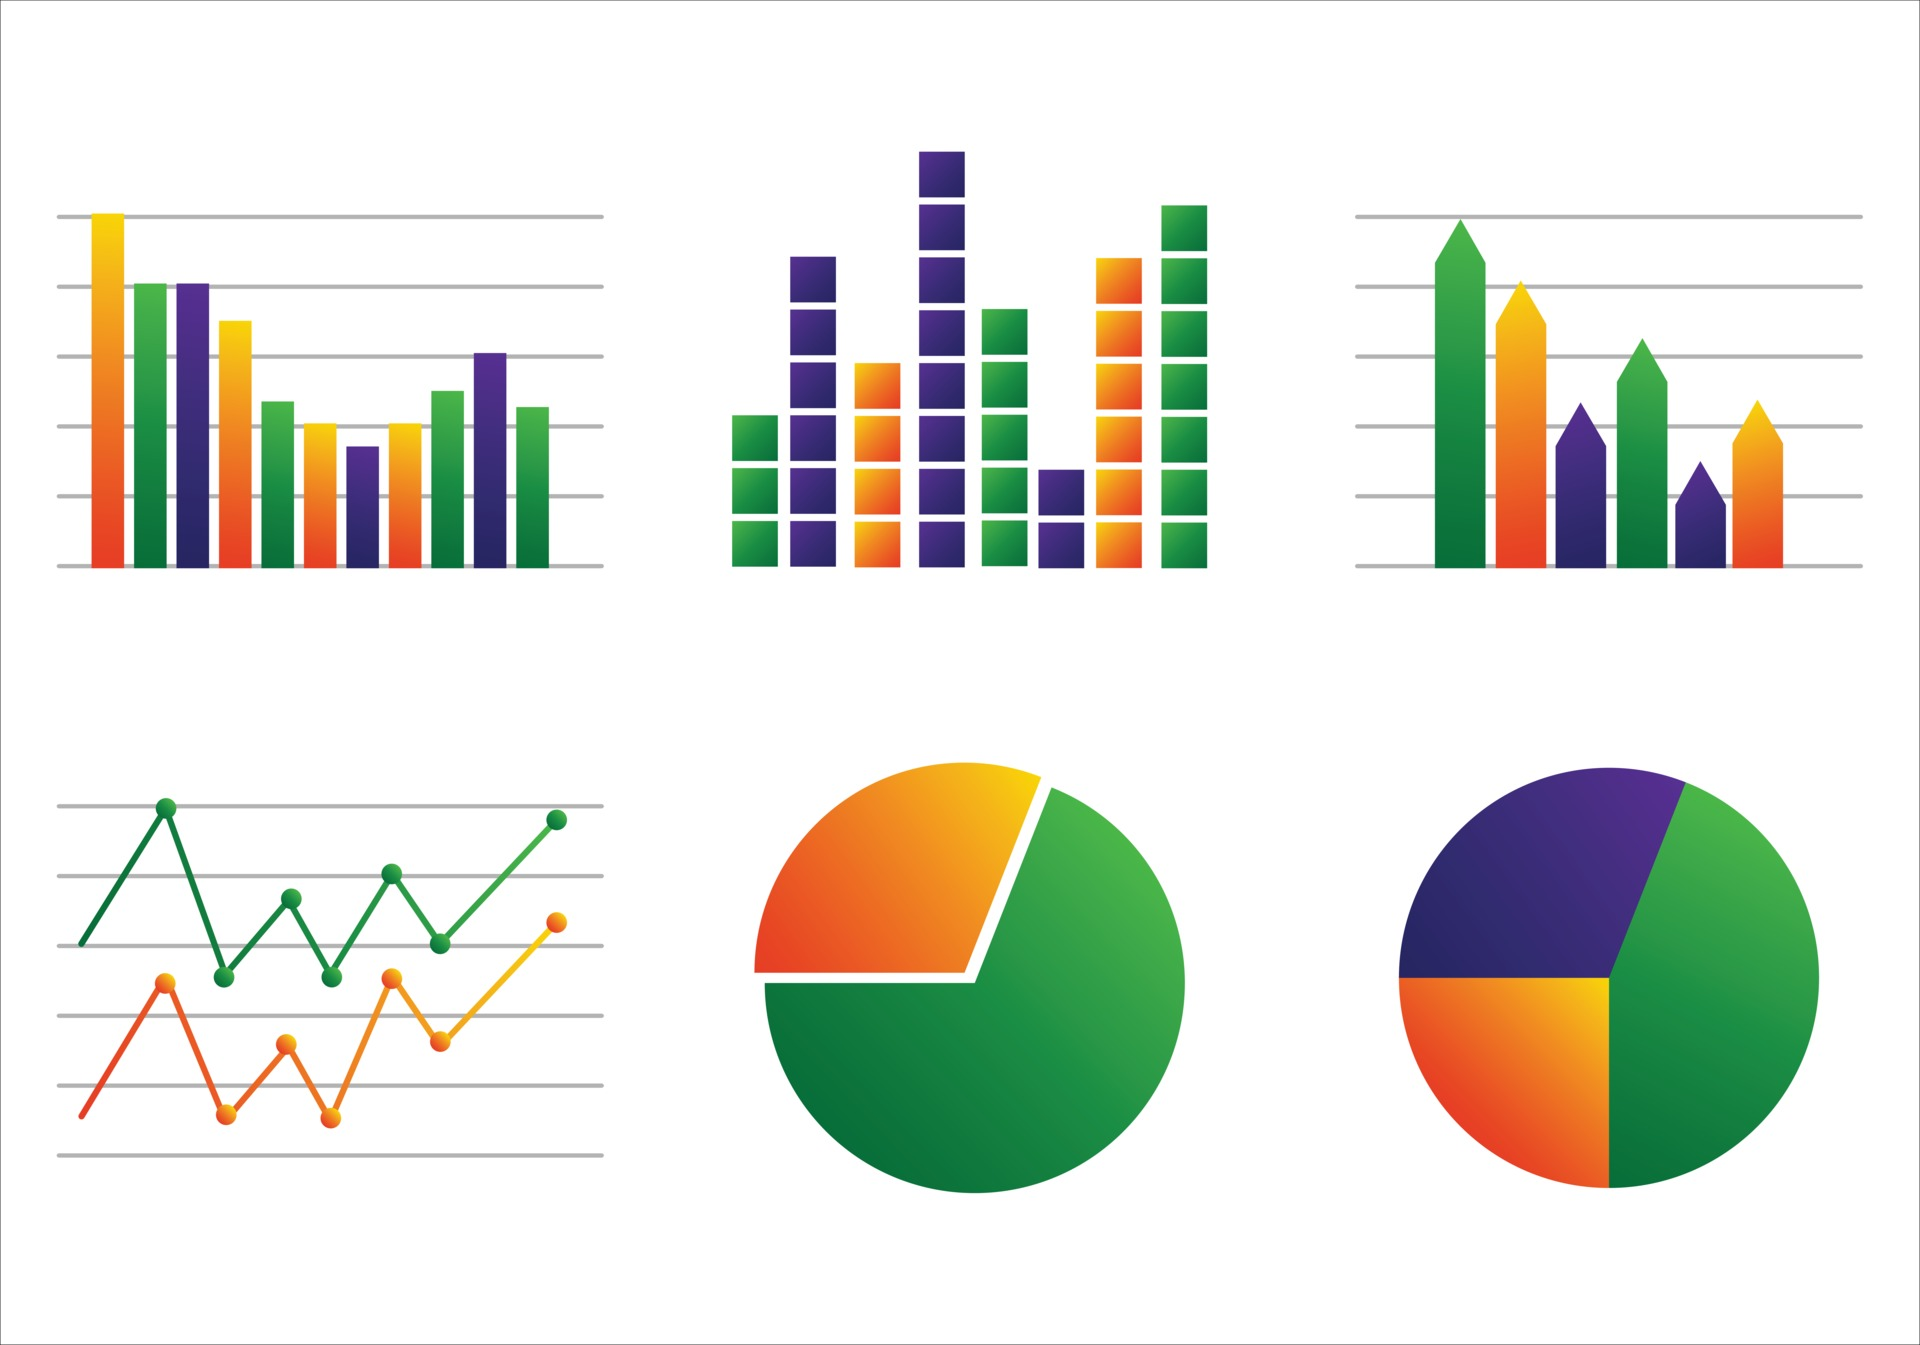
\includegraphics[width=0.8\linewidth]{graph}
\end{figure}
\blindtext

\blindtext \cite{latex2e}.
\begin{figure}[t]
\centering
\caption{Main heading of the figure, with \texttt{[t]}}
\begin{subfigure}{0.48\textwidth}
\caption{Heading of first figure}
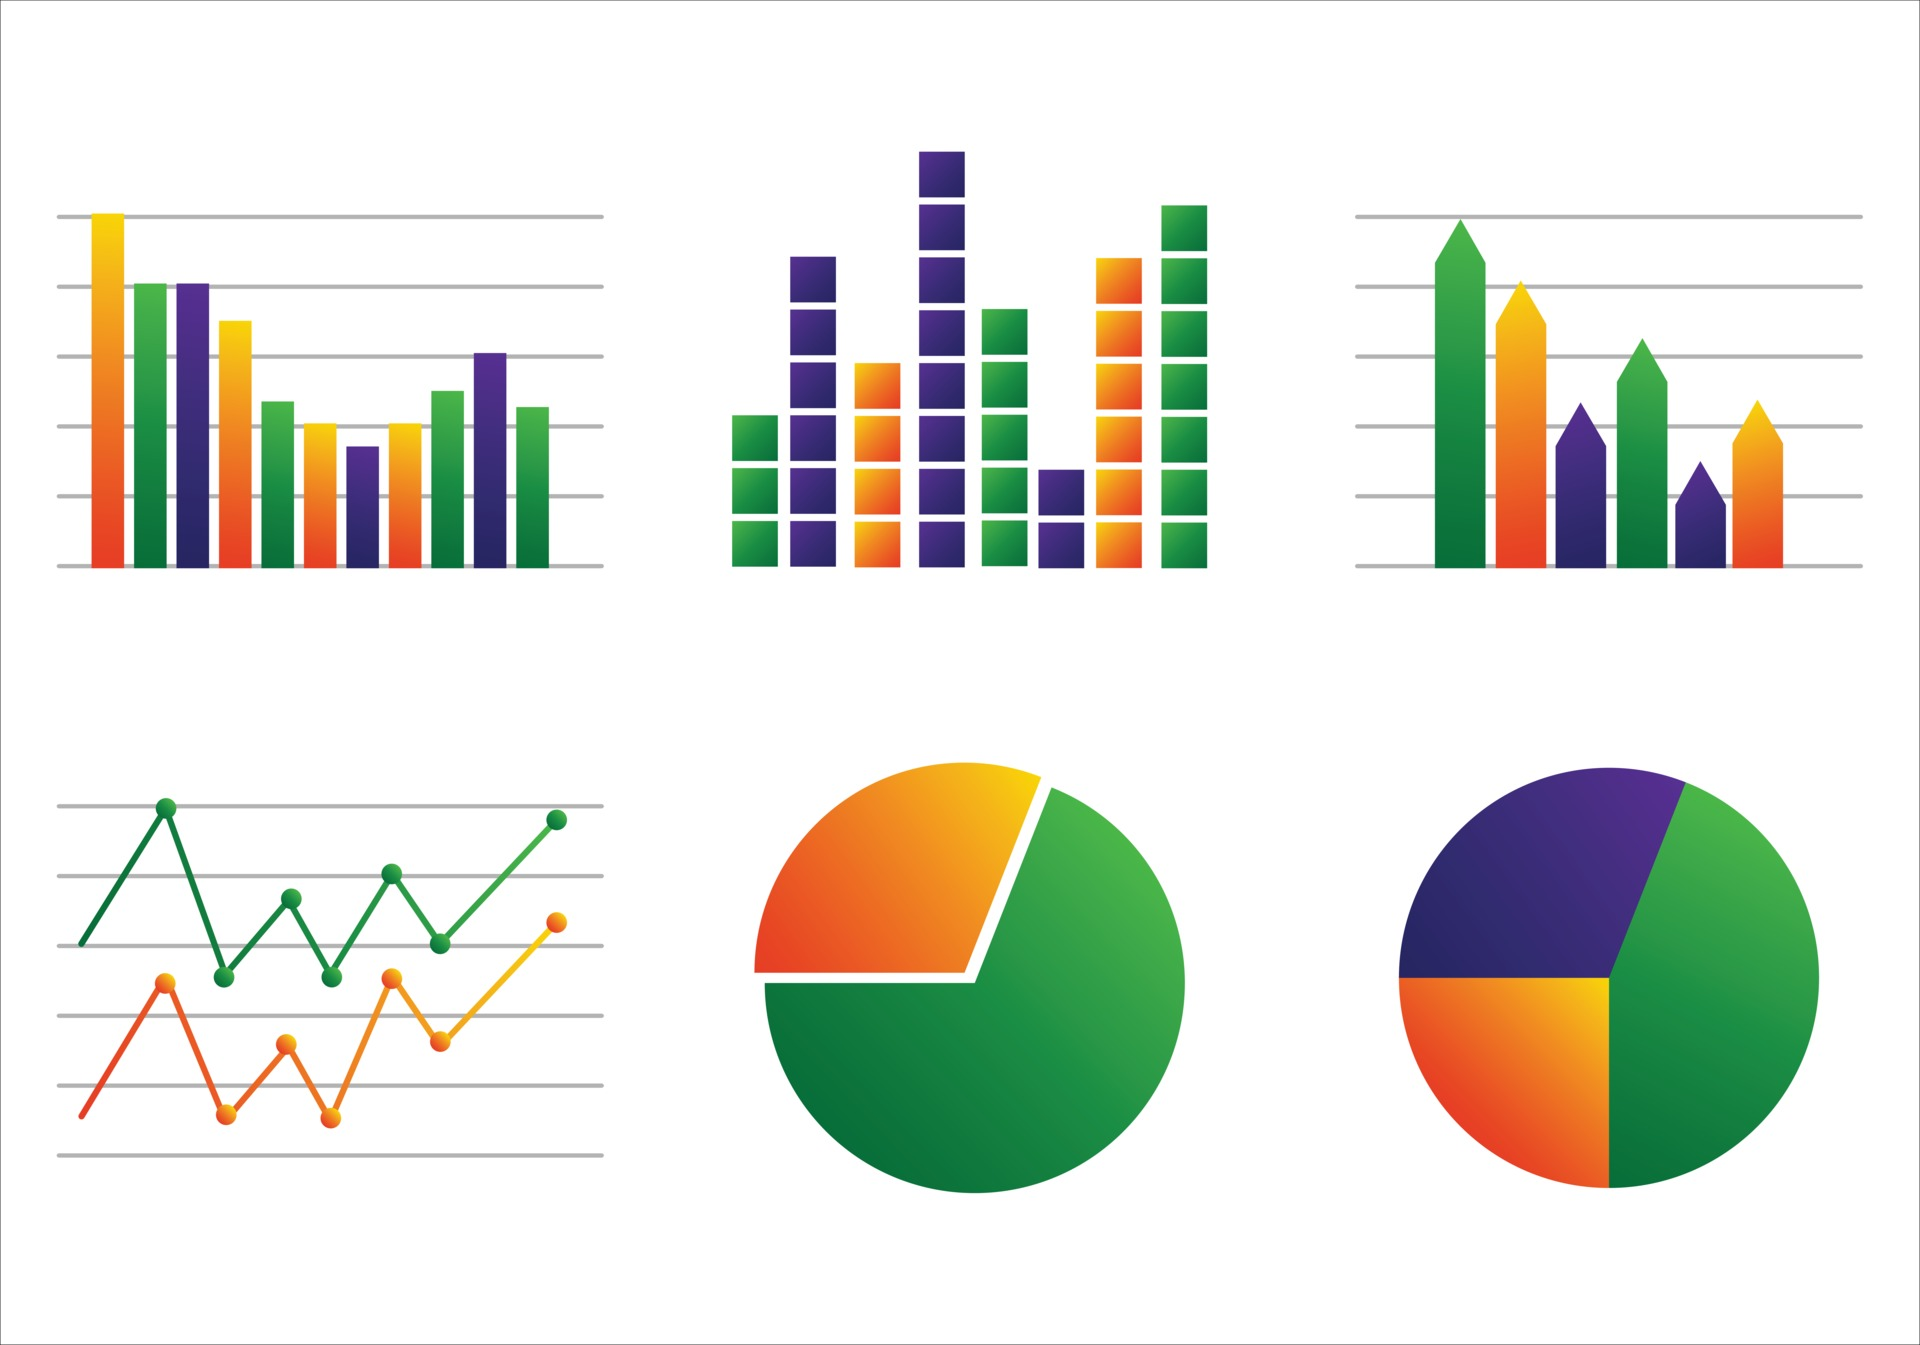
\includegraphics[width=1\linewidth]{graph}
\end{subfigure}
\begin{subfigure}{0.48\textwidth}
\caption{Heading of second figure}
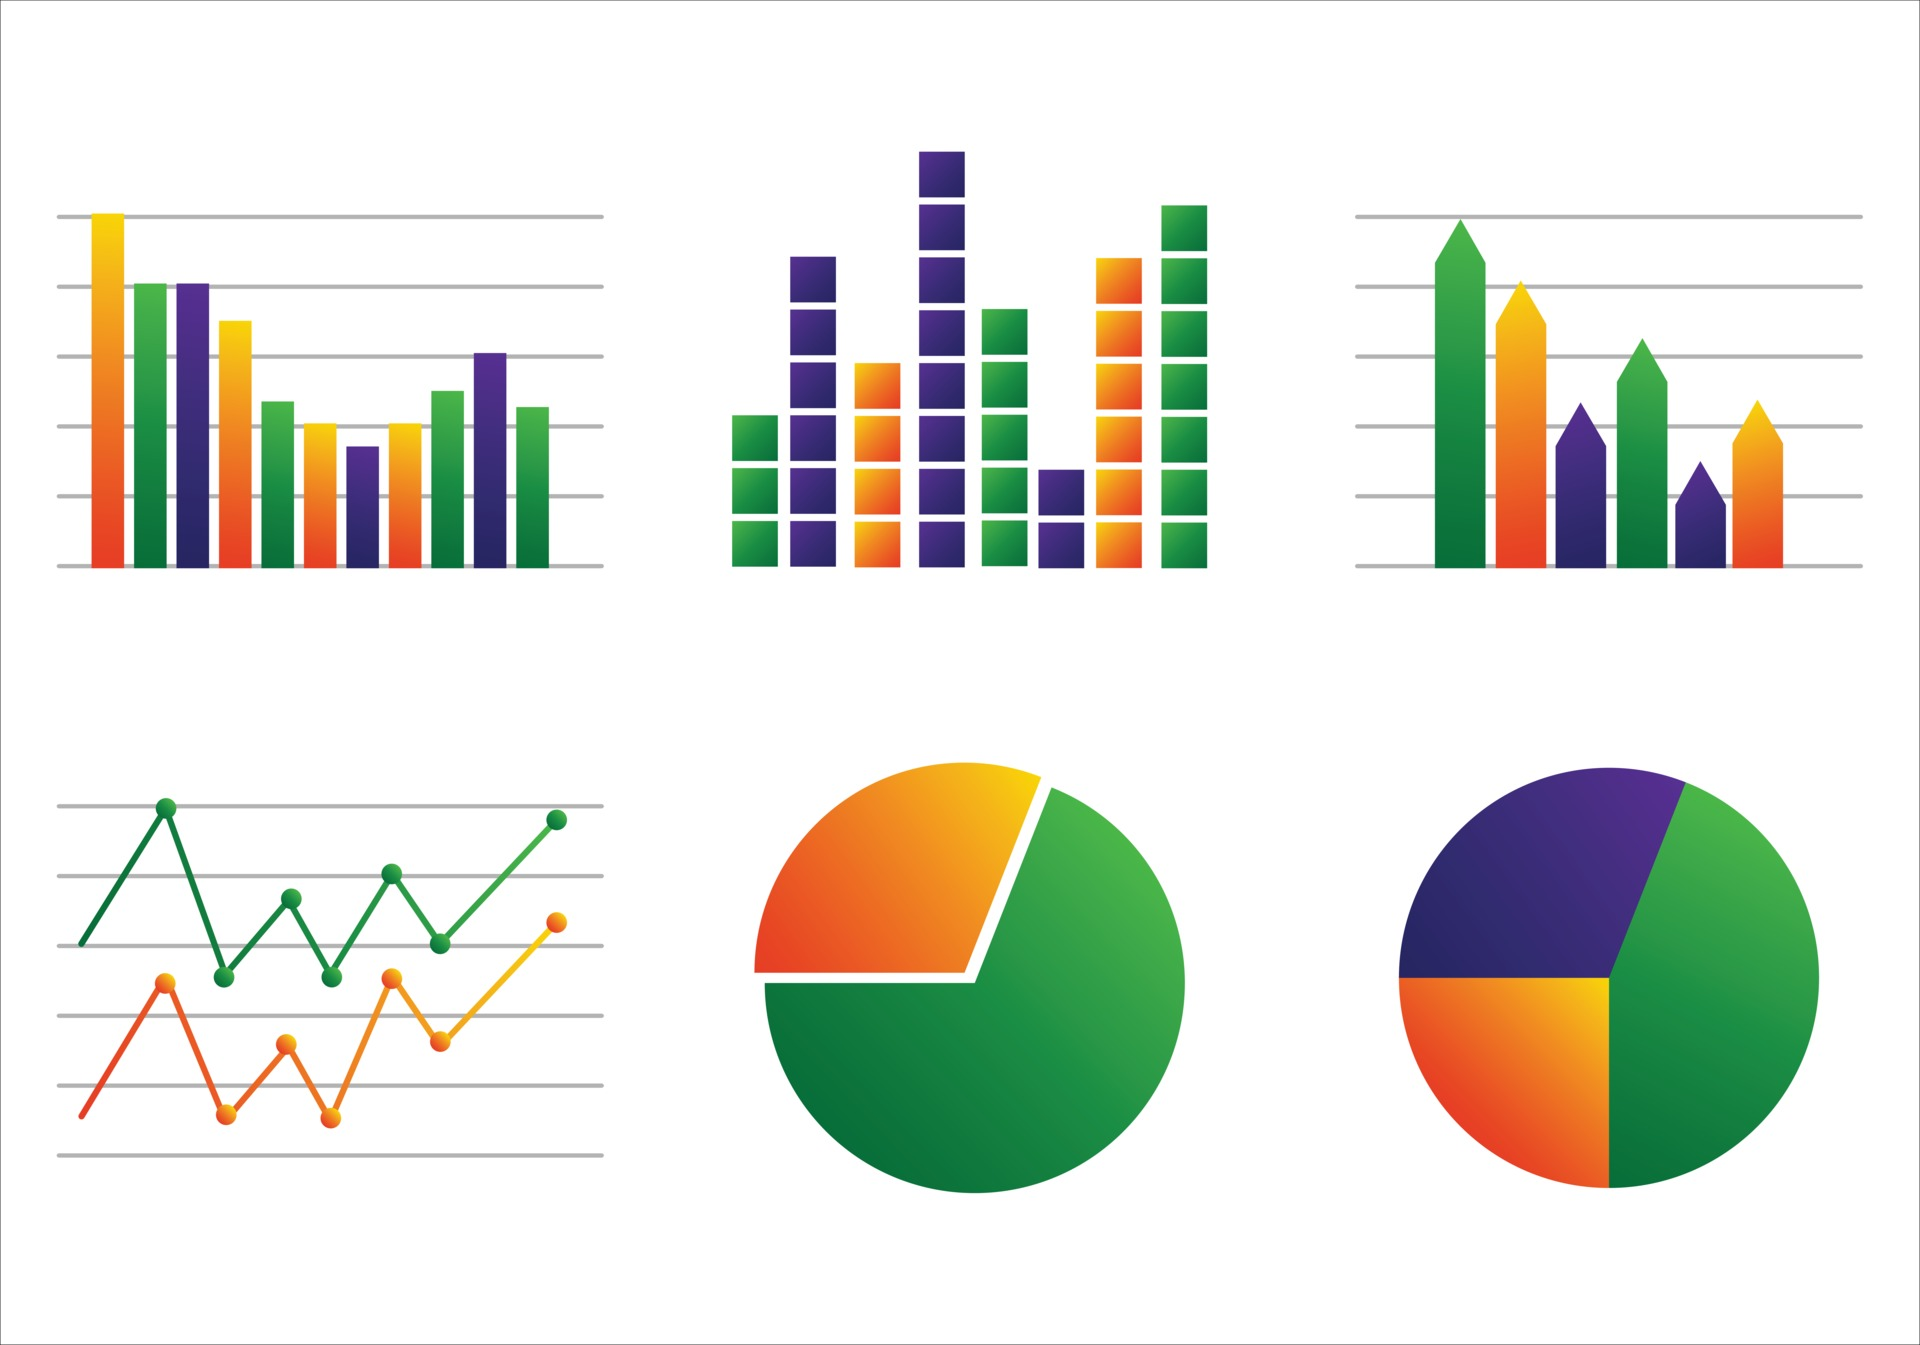
\includegraphics[width=1\linewidth]{graph}
\end{subfigure}
\end{figure}
\blindtext

%%%%%%%%%%%%%%%%%%%%%%%%%%%%%%%%%%%%%%%%%%

\bibliography{biblio}
\bibliographystyle{chicago}

%%%%%%%%%%%%%%%%%%%%%%%%%%%%%%%%%%%%%%%%%%

\section{First section in Appendix}

\blindtext 
\begin{equation}
x = y + z
\end{equation}
\blindtext 

\subsection{Subsection in Appendix}

\blindtext 

\section{Second section in Appendix}

\blindtext 
\begin{equation}
x = y + z
\end{equation}
\blindtext 

%%%%%%%%%%%%%%%%%%%%%%%%%%%%%%%%%%%%%%%%%%

\end{document}
